%-------------------------------------------------------------------------%
\section{Possible decay channels of the top squarks} 
\label{sec:stopDecay}
Just like the SM particles and their decay dictated by known symmetries and conservation laws, the decay of stops is dictated by the parameters and kinematics suggested by MSSM. The mass of stops would significantly affect the decay modes. \\

A heavy enough stop at the order of the sum of the top quark mass and neutralino mass ($m_t+m_{\Tilde{\chi}_1^0}$) would undergo a two-body decay into top quarks with neutralinos: $\Tilde{t}\rightarrow t\Tilde{\chi}_1^0$. In the case where the neutralino is instead the chargino, the decay results in bottom quarks with charginos: $\Tilde{t}\rightarrow b\Tilde{\chi}_1^+$) \cite{boehm2000decays}. A lighter stop that is above the sum of the bottom quark mass, W-boson mass and neutralino mass ($m_b + m_W + m_{\Tilde{\chi}_1^0}$) would imply a three-body decay $\Tilde{t}\rightarrow b W \Tilde{\chi}_1^0$. Four-body decays into a combination of bottom quarks, neutralinos and SM fermions, may also be possible: $\Tilde{t}\rightarrow b\Tilde{\chi}_1^0 f \Bar{f}'$ \cite{boehm2000decays}. However, the four-body decay is only relevant when the two- and three-body decays are kinematically forbidden. This would also allow a flavor-suppressed decay to a charm quark: $\Tilde{t}\rightarrow c\Tilde{\chi}_1^0$ \cite{aad2014search}. \\

An important assumption made in these decays is that the stops are heavier than the neutralino mass ($m_{\Tilde{t}} > m_{\Tilde{\chi}_1^0} $) so that the neutralinos remain the lightest (LSP). Additional decays become apparent when sparticles other than $\Tilde{\chi}_1^0 $ are lighter than the stop, for example, the charginos $\Tilde{\chi}_1^{\pm}$. A diagram from \cite{aad2014search} is shown in Figure \ref{fig:decayMode}, that represent the statements above under the assumption that $ \Tilde{\chi}_1^0 $ and $\Tilde{t}$ are the lightest and next-lightest particles in the MSSM. For this project, we stick to a simplified model where the right-handed\footnote{The SM quarks have a left- and right-handed component in which they are a doublet and a singlet respectively. The MSSM counterpart follows this convention and the mixing of the two states provides two distinct squarks. The doublet allows mixing with other quarks (e.g. tops with the bottom) thus making them more complicated and potentially heavier.} stops mix to form the lighter stop. Furthermore, the decays we explore also follows the simplified model, where our desired background events is the process given by Equation (\ref{eq:background}) and the desired signal events given by Equation (\ref{eq:signal}). The final state includes one charged lepton, some missing energy, and some hadronic jets, one which that originates from the $b$-quark at a minimum, as shown in Figure \ref{fig:stopDecay}.\\


\begin{figure}[htbp]
    \centering
    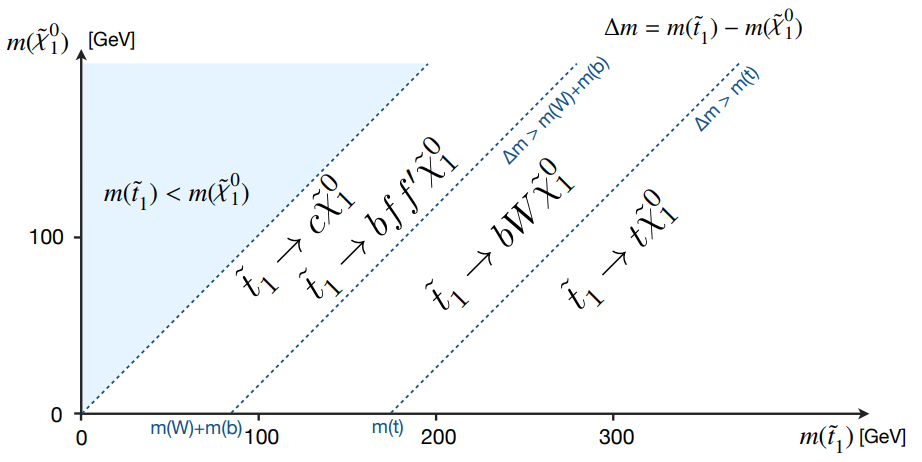
\includegraphics[width=0.75\linewidth]{decaymodes.png}
    \caption{Possible decay modes for stops within the mass-parameter space of $\Tilde{t}_1 $ and $ \Tilde{\chi}_1^0 $ \cite{aad2014search}. The blue filled region is kinematically forbidden due to the neutralino mass being heavier than the stop mass thus resulting in stops that are not energetic enough. As the mass of stops get heavier, the allowed decays differ due to its varying allowed kinematics, favoring on-shell decays over off-shell decays.}
    \label{fig:decayMode}
\end{figure}

\begin{equation}
 pp \rightarrow t \Bar{t} \rightarrow b\Bar{b}jjl\cancel{\it{E}}_{T},
 \label{eq:background}
\end{equation}
\begin{equation}
  pp \rightarrow \Tilde{t}\Tilde{t^*} \rightarrow t \Bar{t} \Tilde{\chi^0_1}\Tilde{\chi^0_1} \rightarrow b\Bar{b}jjl\cancel{\it{E}}_{T},
  \label{eq:signal}
\end{equation}

\begin{figure}[htbp]
    \centering
    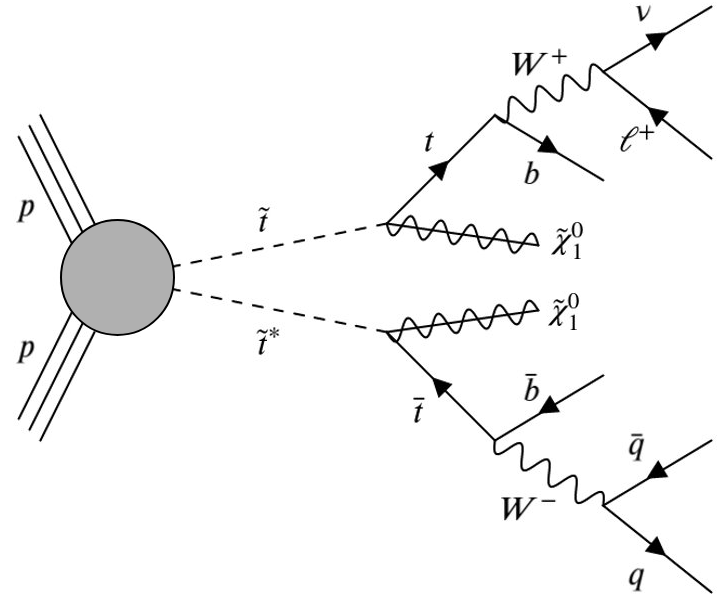
\includegraphics[width=0.5\linewidth]{stop_decay2.png}
    \caption{Decay chain of the signal of interest $\Tilde{t}\Tilde{t}^* \rightarrow t\bar{t}\Tilde{\chi}_1^0\Tilde{\chi}_1^0 $ with a final of state of one charged lepton and hadronic jets originating from the quark-antiquark pair and bottom quarks.}
    \label{fig:stopDecay}
\end{figure}
%-------------------------------------------------------------------------%
%\section{Mass of the top squark}
%\label{sec:stopMass}
%The mass eigenstates for the top squarks are given by the equation

%\begin{align}
%    \begin{pmatrix} \Tilde{t}_1 \\ \Tilde{t}_2 \end{pmatrix} = 
%    \begin{pmatrix} \cos\theta_\Tilde{t} & -\sin\theta^*_\Tilde{t} \\ \sin\theta_\Tilde{t} & \cos\theta^*__\Tilde{t} \end{pmatrix}
%    \begin{pmatrix} \Tilde{t}_L \\ \Tilde{t}_R \end{pmatrix}
%    \label{eq:stopMass}
%\end{align}
%where $ \theta_\Tilde{t} $ is the stop mixing angle in the range $ 0 \leq {\theta_\Tilde{t}} \leq \pi $ satisfying $ |\cos\theta_{\Tilde{t}}|^2 + |\sin\theta_{\Tilde{t}}|^2 = 1 $ \cite{martin1997supersymmetry}. \\

%The mass splitting of the two stops $ \tilde{t}_1 $ and $ \tilde{t}_2 $ arise from the squared-mass matrix for stops, where the off-diagonal elements involves a large top-quark Yukawa coupling ($y_t$ term) that induces such a phenomena \cite{kraml2016scalar}. Diagonalizing gives the $\Tilde{t}_L$ and $\Tilde{t}_R$ components on the right-hand side of Equation (\ref{eq:stopMass}). One possible model in the MSSM predicts that $\Tilde{t}_1$ is the lightest of all squarks predominantly theorized to be $\Tilde{t}_R$ which is the right-handed stops \cite{martin1997supersymmetry}. Although there has been no success in the direct detection of the particle, experimental efforts have been made to set constraints on its mass \cite{kraml2016scalar, aad2014search, abdughani2018probing, sirunyan2018search, yoshihara2017search}.

%-------------------------------------------------------------------------%
\section{Mass parameters for the top squarks and neutralinos}
Experiments at the Large Hadron Collider have set limits on the stop mass and neutralino mass since the operation began in 2008. Many searches involving other exotic particles and its properties have been performed, thus how do particle physicists create such limits, and in the lucky scenario such as the Higgs boson, claim a discovery? In short, a frequentist approach\footnote{A Bayesian approach can also be taken, where it makes use of the posterior probability known as Bayes' theorem. It is said to have a wider range of applicability due to its ability to account for unknown parameters which frequentist approaches cannot, and differs greatly in its interpretation when claiming a discovery \cite{lista2017statistical}.} can be taken where the statistical analysis relies on likelihood-based hypothesis testing.

%-------------------------------------------------------------------------%
\subsection{Frequentist statistics - setting limits in searches}
\label{sec:freqStat}
A likelihood function provides us with the probability distribution function evaluated for the observed data, in which the extended likelihood function to account for the Poisson distribution of the number of events $N$ is given by
\begin{equation}
    L(\vec{x}_1,...,\vec{x}_n; \vec{\theta}) 
    = \frac{e^{-\mu_n(\vec{\theta})}\mu_n(\vec{\theta})}{n!}\prod^n_{i=1} f(\vec{x}_i;\vec{\theta})
    \label{eq:genLikelihood}
\end{equation}
where $\vec{x}_i$ is an individual observation in a set of $i=1,...,n$ random variables amongst $N$ number of uncorrelated events, $\mu_n(\vec{\theta})$ is the expected number of events dependant on some nuisance parameter $\vec{\theta}$, a parameter in which unknown parameters coupled to the parameter of interest from detector response is accounted for \cite{lista2017statistical}. When a background-only hypothesis $H_0$ is given as $\mu_n(\vec{\theta})=b$, then the alternate hypothesis  $H_1$ includes both signal and background events such that $\mu_n(\vec{\theta})=\mu s+b$. The likelihood function (\ref{eq:genLikelihood}) is then a parameter of $\mu$ i.e. $L(\mu,\vec{\theta})$, with $\mu=0$ corresponding to $H_0$ and $\mu=1$ to $H_1$. \\

We can obtain the profile likelihood ratio for the evaluated hypotheses with $H_0 \rightarrow L_{s+b}$ and $H_1 \rightarrow L_b$ into
\begin{equation}
    \lambda(\mu) = \frac{L_{s+b}(\mu, \hat{\hat{\theta}})}{L_b(\hat{\mu},\hat{\theta})}
    \label{eq:genLR}
\end{equation}
for some maximum-likelihood estimators\footnote{The maximum likelihood estimators provide the parameter values that maximize the search for a particular observation within the set.} $\hat{\mu}$ and $\hat{\theta}$, and $\hat{\hat{\theta}}$ being the conditional maximum-likelihood estimator \cite{cowan2011asymptotic}. The value for $\lambda$ rests between the range $0 \leq \lambda \leq 1$ which can be applied for some test statistic $q_\mu$\footnote{The signal discovery test statistic is $q_0$ where it holds the value $-2 \ln \lambda (0)$ for $\hat{\mu}=0$ and zero otherwise.} defined as
\begin{equation}
    q_\mu = \left\{
        \begin{array}{ll}
            -2\ln \lambda(\mu) & \quad \hat{\mu} \leq \mu \\
            0 & \quad \hat{\mu} \geq \mu
        \end{array}
    \right.
\end{equation}
where the larger the value $q_\mu$ is, the more likely the hypothesis whose value is represented by $\mu$ is incompatible with the data. This allows us to compute the significance\footnote{For a discovery to be claimed, particle physicists require a minimum of $Z=5$ that corresponds to $p=2.87\times10^{-7}$ when rejecting the background only hypothesis.} $Z$ and its associated $p$-value with the relationship
\begin{equation}
    Z = \Phi^{-1}(1-p) = \sqrt{q_\mu}
    \label{eq:Z}
\end{equation}
The exclusion of the hypothesis $\mu$ is supported when a threshold $p=\alpha$ is applied with a low value e.g. $\alpha=0.05$ for a 95\% confidence level ($Z=1.64$) \cite{cowan2011asymptotic}. \\

Collider experiments are considered a form of counting experiments, thus the observed events are categorized under a Poisson distribution with a mean of $\mu_s+\mu_b$ where $\mu_{s(b)}$ is the estimated number of signal(background) \cite{lista2017statistical, adam-bourdarios_learning_2014}. This gives us a more simplified version to Equation (\ref{eq:genLikelihood});
\begin{equation}
    P(n|\mu_s,\mu_b) = \frac{(\mu_s+\mu_b)^n}{n!}e^{-(\mu_s+\mu_b)}
    \label{eq:Poisson}
\end{equation}
whose likelihood ratio is given by
\begin{equation}
    \lambda = \frac{P(n|\mu_s,\mu_b)}{P(n|\hat{\mu_s},\mu_b)}
    \label{eq:likelihoodRatio}
\end{equation}
where $\hat{\mu_s}$ is the maximum likelihood estimator of $\mu_s$. \\


%-------------------------------------------------------------------------%
\subsection{Exclusion limits for the stop and neutralino masses}
The exclusion of masses for new exotic particles are performed according to rigorous statistic that Section \ref{sec:freqStat} has only touched a small portion of. The exclusion of stop and neutralino masses is visually presented as an exclusion curve in CMS and ATLAS, such as those seen in Figure \ref{fig:limits} \cite{cms2019search} where \textit{inside} the expected limit (in red) and observed limit (in black) have already been searched for and excluded. \\

\begin{figure}[htbp]
    \centering
    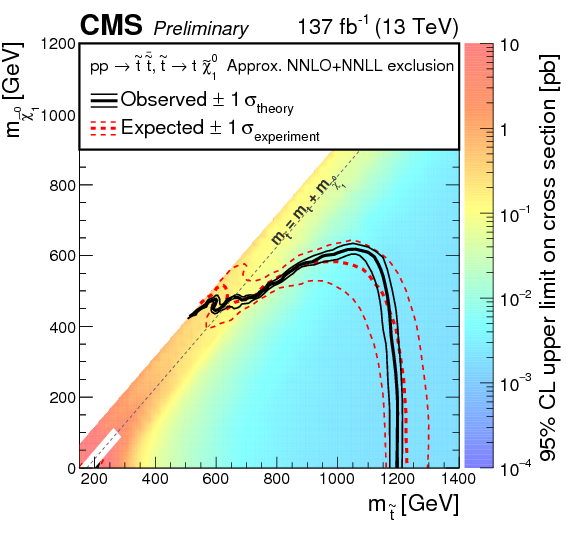
\includegraphics[width=12cm, height= 12cm]{stop_limits.png}
    \caption{The latest cross-section and mass limits for the process $\Tilde{t}\Tilde{t}^* \rightarrow t\bar{t}\Tilde{\chi}_1^0\Tilde{\chi}_1^0 $ set by the CMS experiment \cite{cms2019search}. Inside the black curve is the observed excluded masses for stops and neutralino, and outside this line remains a plausible region for masses for these particles, with the stop mass' limit pushed to the TeV scale. According to the color bar, the further out into to parameter space we travel to, the allowed cross-section is allowed.}
    \label{fig:limits}
\end{figure}

In this particular figure, it is presented that the expected limit to the process $pp \rightarrow \tilde{t}\tilde{t}^* \rightarrow t\tilde{\chi}_1^0$ falls under that of the observed limit when both masses are high i.e. when stop masses are in the order of $1\sim1.2$TeV and neutralino masses in the order of $\sim600$ GeV. It is also shown that the observed limit falls under the expected limit when the mass there is a massive mass difference between the stop and the neutralino i.e. $m_{\tilde{\chi}_1^0}\ll m_{\tilde{t}}$. These two points indicated that a large mass difference between the two particles can is preferred at the current limits. Furthermore, the upper limit on the cross-section for the production of this process is provided in color-code, such that the values that fall above cross-sections and its corresponding colour will be excluded. This implies that our signal selection efficiency is high when searching in regions with weaker limits. \\

The path sitting around $ m_{\tilde{t}} \approx 1.2$ TeV is an interesting path to follow, and observe how the algorithms (in which this will be discussed in detail in a later section) perform. In addition, reference \cite{roxlo2018opening} have explored the performance of their neural networks discriminating stop production to top production, albeit in a dilepton final state within the $\tilde{t} \rightarrow t \tilde{\chi}_1^0$ decay. Their choice of mass parameters are set as the parameters our fourth benchmark explores: $m_{\tilde{t}} =750$ GeV and $m_{\tilde{\chi}_1^0} = 1$ GeV, well within the exclusion limit in Figure \ref{fig:limits}. Table \ref{tab:benchmarks} shows a summary of mass parameters chosen to explore. In particular, it would be interesting to observe the behavior of the classifiers when the deviation for stop masses is slight opposed to a large deviation in neutralino masses. Intuitively, the large difference would imply that the final states will carry a large excess of missing energy, thus allowing the algorithm to distinguish them easily and allowing us to observe the physical behavior. 

\begin{table}[htbp]
    \centering
    \begin{tabular}{c|c|c|c} 
    \toprule
    Benchmark No. & Position & $m_{\Tilde{t}}$ (TeV) & $m_{\Tilde{\chi}_1^0}$ (GeV) \\
    \midrule
    \rowcolor{gray!6} 1 & Outside & $ 1.2 $ & $ 600 $ \\
    2 & Outside & $ 1.225 $ & $ 400 $ \\
    \rowcolor{gray!6} 3 & Outside & $ 1.25 $ & $ 100 $ \\
    4 & Inside & $ 0.75 $ & $ 1 $\\
    \bottomrule
    \end{tabular}
    \caption{Chosen parameters for building classifiers, three of which tracing just outside of the observed exclusion limit in Figure \ref{fig:limits}, and one of which is completely inside the curve, following that of \cite{roxlo2018opening}. In doing so we observe how the mass difference between the stops and neutralinos affect the production and sensitivity.} 
    \label{tab:benchmarks}
\end{table}

